\chapter{Estado de arte}



Neste capitulo pretende-se apresentar algumas das possíveis tecnologias de utilização nesta. 




\section{Sistema de gestão de base de dados (\ac{SGBD})}


\subsection{PostgreSQL}

\subsection{MySQL}

\subsection{SQL server}



\subsection{Comparação e solução adotada}


No entanto, é pertinente fazer uma comparação entre o PostgreSQL e
outras ferramentas open-source como o MySQL. Embora as diferenças entre
as duas ferramentas não sejam muito grandes, podemos ter também em conta
a performance de uma e outra. Uma comparação feita usando o benchmark
TPC-H 8 mostra que a performance do PostgreSQL é ligeiramente superior à
do MySQL na maioria das queries [22].



\newpage
\section{Desenvolvimento web}



Para o desenvolvimento da dashboard poderiam ser adotadas duas estratégias distintas para o desenvolvimento web: 

\begin{itemize}
	\item Manipulação local usando \ref{JS} do DOM. 
\end{itemize}



Neste contexto poderiam ser utilizados 


Angular, React

Servidor serve conteudos criados em função dos pedidos do cliente 



\subsection{Django}


\subsection{Faslk}

\subsection{ASP.net}



\subsection{Conclusões e solução adotada}



\newpage
\section{Desenvolvimento mobile}



\subsection{Plataformas nativas}




\subsection{Multi-plataforma}

http://websocialdev.com/lista-de-frameworks-para-desenvolvimento-mobile/


\subsection{Conclusões e solução adotada}





\newpage
\section{REST Frameworks}




\subsection{Django Rest Framework}





Django REST Framework é uma ferramenta considerada 'poderosa e flexível para a construção de APIs Web' [], que pode ser usada juntamente com a framework de desenvolvimento de aplicações Web Django, que quando integrada no desenvolvimento de um determinado \textit{backend} permite a implementação de serviços do tipo REST.



A API navegável Web é uma vitória usabilidade enorme para os desenvolvedores.

Políticas de autenticação , incluindo pacotes para OAuth1a e OAuth2 .

Serialização que suporta tanto ORM e não ORM fontes de dados.

Customizável todo o caminho - basta usar vistas regulares baseadas na função , se você não  precisar dos mais poderosos recursos .

Extensa documentação , e grande apoio da comunidade .

Utilizado e confiável por empresas internacionalmente reconhecidas, incluindo Mozilla , 
Red Hat , Heroku , e Eventbrite .




\subsection{Flask-RESTful}

\subsection{Conclusões e solução adotada}




com autenticação via token 


\section{Documentação automática}

\subsection{Documentação API}

utilizado swagger; apenas permite acesso a quem está logado... incorporar layout do swagger com o do salidashboard




app mobile
microcontroladores -> controller modulers 


documentação com swager 





\newpage
\section{Sensores}


Esta secção tem como objetivo fazer um estudo comparativo entre diferentes tecnologias usadas para a medição dos vários parâmetros ambientais necessários ao controlo e monitorização da salicornia. Todas as soluções adaptadas tem termos de hardware escolhidas devido à possui-las. 

\subsection{Sensor de temperatura }
Existem vários tipos de sensores de temperatura baseados em princípios de funcionamento distintos. 


\begin{itemize}
	\item \textbf{Termopares}: 
	\item \textbf{RTDs}:
	\item \textbf{Termístor}: 
	\item \textbf{Circuito integrado}: 
\end{itemize}




\subsubsection{Solução adotada}


TTC 104

\begin{figure}[h]
	\centering
	\begin{minipage}[b]{0.3\textwidth}
		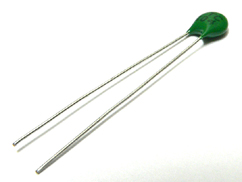
\includegraphics[width=\textwidth]{img/hardware/temperatura.jpg}
		\caption{Flower one.}
	\end{minipage}
	\hfill
	\begin{minipage}[b]{0.3\textwidth}
		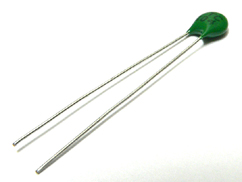
\includegraphics[width=\textwidth]{img/hardware/temperatura.jpg}
		\caption{Flower two.}
	\end{minipage}
\end{figure}



\begin{table}[h]
	\centering
	
	\begin{tabular}{|
			>{\columncolor[HTML]{C0C0C0}}c |c|} \hline
		Resistencia & isso \\ \hline
		Valor máximo & isso \\ \hline
		Valor minimo & isso \\ \hline
		Nome & isso \\ \hline
	\end{tabular}
	\caption{Características do sensor TTC 104}
	\label{my-label}
\end{table}





\newpage

\subsection{Sensor de luminosidade (GL5528)}


O LDR (Light Dependent Resistor) é um componente cuja resistência varia de acordo com a intensidade da luz. Quanto mais luz incidir sobre o componente, menor a resistência. Este sensor de luminosidade pode ser utilizado em projetos com arduino e outros microcontroladores para alarmes, automação residencial, sensores de presença e etc.




\subsubsection{Solução adotada}

\begin{figure}[h]
	\centering
	\begin{minipage}[b]{0.4\textwidth}
		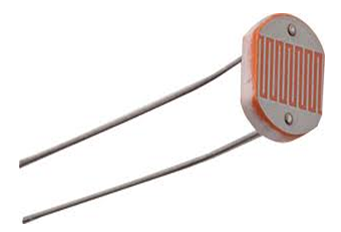
\includegraphics[width=\textwidth]{img/hardware/luminosidade.png}
		\caption{Flower one.}
	\end{minipage}
	\hfill
	\begin{minipage}[b]{0.4\textwidth}
		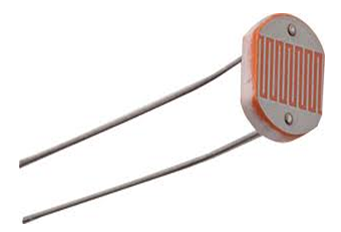
\includegraphics[width=\textwidth]{img/hardware/luminosidade.png}
		\caption{Esquema eletrotécnico}
	\end{minipage}
\end{figure}











\begin{table}[h]
	\centering
	
	\begin{tabular}{|
			>{\columncolor[HTML]{C0C0C0}}c |c|} \hline
		Diâmetro & 5mm \\ \hline
		Tensão máxima & 150VDC \\ \hline
		Potência máxima:& 100mW \\ \hline
		Tensão de operação: & -30 C a 70 C \\ \hline
		Espectro: &540nm \\ \hline
		Comprimento com terminais:& 32mm \\ \hline
		Resistência no escuro: &1 M (Lux 0) \\ \hline
		Resistência na luz: &10-20 Komega (Lux 10) \\ \hline
	\end{tabular}
	\caption{Características do sensor GL5528}
	\label{my-label}
\end{table}


\newpage
\subsection{Sensor de nível líquido}


Water Level Switch Liquid Level Sensor Plastic Ball Float


\begin{figure}[h]
	\centering
	\begin{minipage}[b]{0.4\textwidth}
		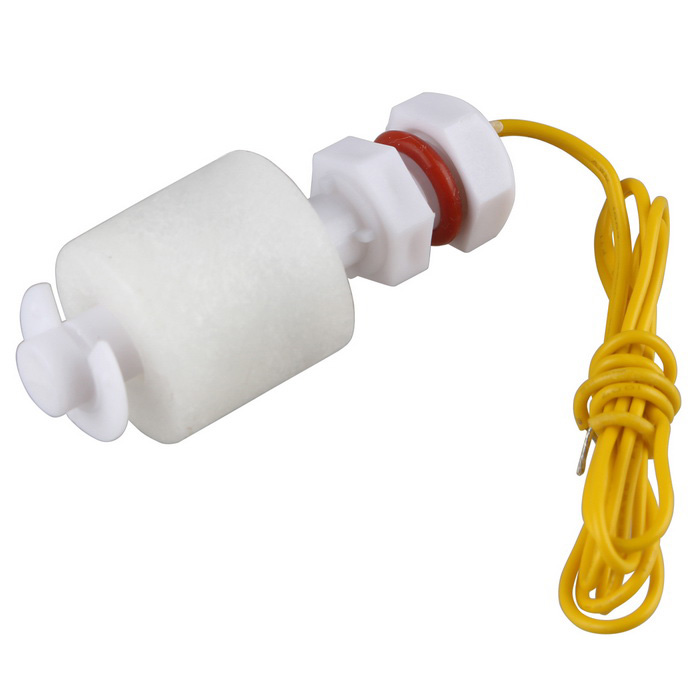
\includegraphics[width=\textwidth]{img/hardware/liquido.JPG}
		\caption{Flower one.}
	\end{minipage}
	\hfill
	\begin{minipage}[b]{0.4\textwidth}
		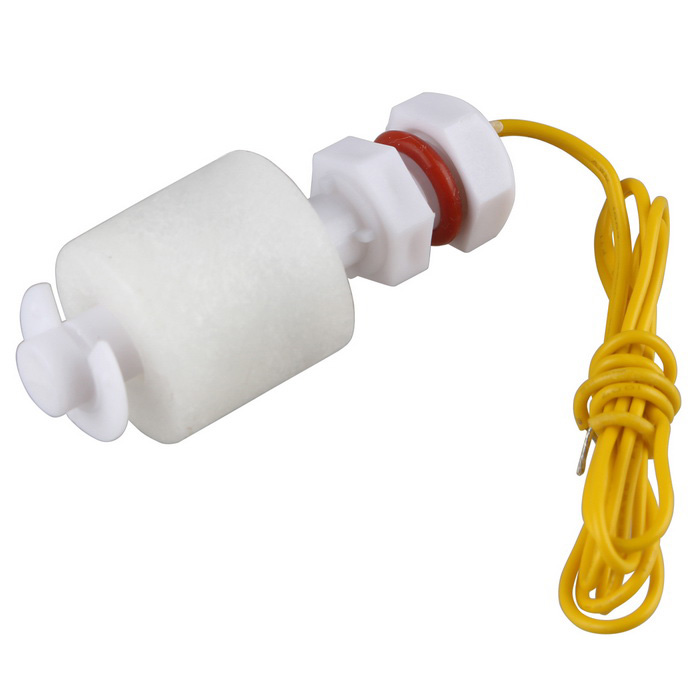
\includegraphics[width=\textwidth]{img/hardware/liquido.JPG}
		\caption{Flower two.}
	\end{minipage}
\end{figure}


\newpage

\subsection{Simulador de bomba para transferências de águas (led)}


dsadsa

\begin{figure}[h]
	\centering
	\begin{minipage}[b]{0.4\textwidth}
		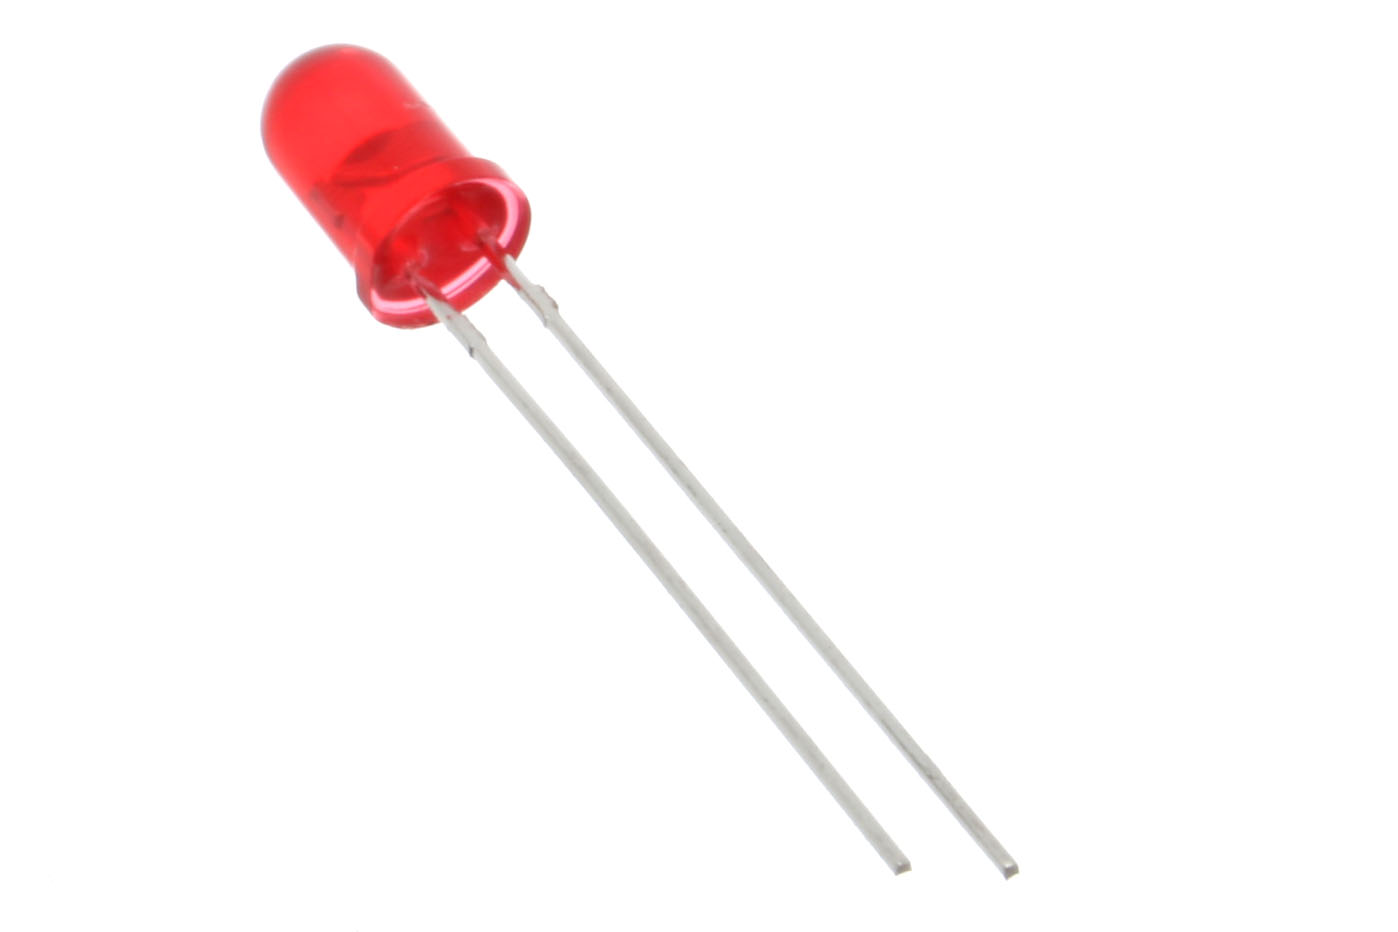
\includegraphics[width=\textwidth]{img/hardware/led.jpg}
		\caption{Flower one.}
	\end{minipage}
	\hfill
	\begin{minipage}[b]{0.4\textwidth}
		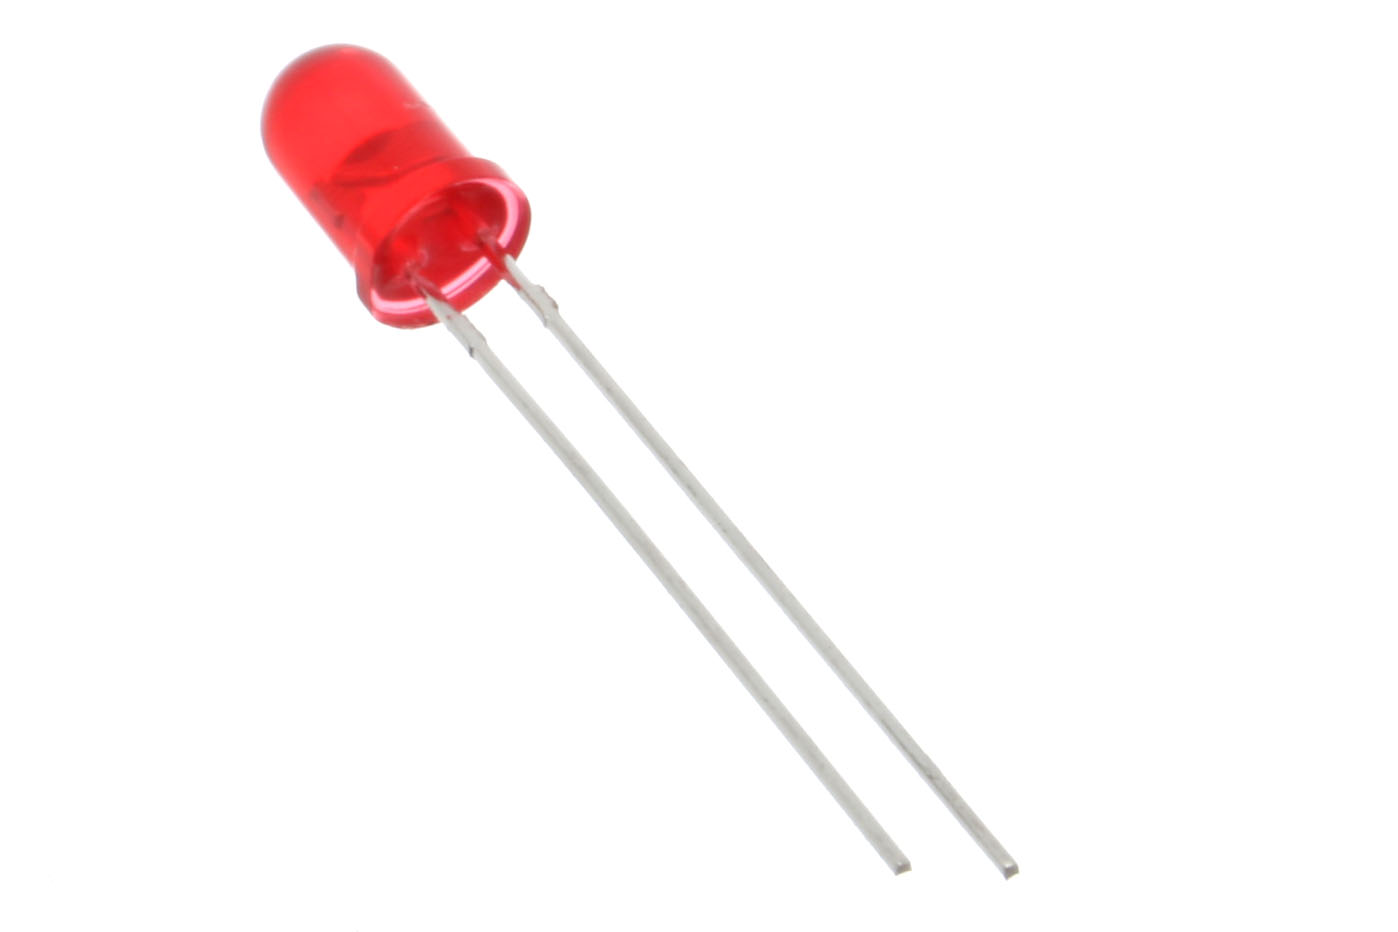
\includegraphics[width=\textwidth]{img/hardware/led.jpg}
		\caption{Flower two.}
	\end{minipage}
\end{figure}




\newpage


\section{Tecnologias de comunicação usadas em \ac{IoT}}

Nesta secção serão apresentados alguns das tecnologias de comunicação mais utilizados em \textit{Internet of Things} que permite a troca de informações entre dispositivos e respetiva comparação entre eles. 



\subsection{RFID/NFC}

A identificação por radiofrequência, conhecida por tecnologia \ac{RFID}, é um método de identificação automático através de sinais de rádio. Consiste essencialmente no armazenamento e posterior envio de informação por meio de ondas electromagnéticas para circuitos integrados compatíveis em rádio frequência.  
Os actuais sistemas de \ac{RFID} possuem grande capacidade de identificação e localização de bens ou pessoas levou, o que fez com que esta tecnologia começasse assumisse um papel importante na indústria e no comércio. A comunicação é efetuada entre uma etiqueta, ou marca, e um leitor.


De forma conceptual, o leitor \ac{RFID} é responsável por transmitir um sinal de rádio através da antena para a tag, e esta responde emitindo para o leitor \ac{RFID} o seu \ac{UID}.


\subsection{Bluetooth}

Bluetooth é uma especificação de rede sem fio de âmbito pessoal (Wireless personal area networks – PANs) consideradas do tipo PAN ou mesmo WPAN


\subsection{WiFi}

rede sem fio IEEE 802.11, que também são conhecidas como redes Wi-Fi ou wireless, foram uma das grandes novidades tecnológicas dos últimos anos. Atuando na camada física, o 802.11 define uma série de padrões de transmissão e codificação para comunicações sem fio, sendo os mais comuns: FHSS (Frequency Hopping Spread Spectrun), DSSS (Direct Sequence Spread Spectrum) e OFDM (Orthogonal Frequency Division Multiplexing). Atualmente, é o padrão de fato em conectividade sem fio para redes locais. Como prova desse sucesso pode-se citar o crescente número de Hot Spots e o fato de a maioria dos computadores portáteis novos já saírem de fábrica equipados com interfaces IEEE 802.25. A Rede IEEE possui como principal característica transmitir sinal sem fio através de ondas!


\subsection{Zigbee}

Zigbee designa um conjunto de especificações para a comunicação sem-fio entre dispositivos eletrônicos, com ênfase na baixa potência de operação, na baixa taxa de transmissão de dados e no baixo custo de implementação. Tal conjunto de especificações define camadas do modelo OSI subsequentes àquelas estabelecidas pelo padrão IEEE 802.15.4.


\subsection{LoRa}

A tecnologia Lora

Wide-Area Network Low-Power ( LPWAN ) ou Low-Power Rede ( LPN ) é um tipo de telecomunicações sem fio de rede projetada para permitir comunicações de longo alcance em uma baixa taxa de bits entre as coisas (objetos relacionados), tais como sensores operados em uma bateria.

As tecnologias WAN de baixa potência são projetadas para ambientes de rede máquina a máquina (M2M). Com a diminuição dos requisitos de energia, maior alcance e menor custo do que uma rede móvel, os LPWANs são pensados para permitir uma gama muito mais ampla de aplicativos M2M e Internet of Things (IoT), que foram limitados por orçamentos e problemas de energia.



\subsection{Sigfox}

Uma empresa francesa que constrói redes sem fio para conectar objetos de baixa energia, como medidores de energia elétrica , smartwatches e máquinas de lavar, que precisam estar continuamente ligados e emitindo pequenas quantidades de dados. Sua tecnologia é voltada para a Internet das Coisas (IoT).



\subsection{GPRS/GSM}


O \ac{GPRS} é uma tecnologia que aumenta as taxas de transferência de dados nas redes \ac{GSM} existentes. 


Vantagens em relação ao GSM


\subsection{Comparação de tecnologias de comunicação}





\subsection{Módulo bluetooth}


\begin{figure}[h]
	\centering
	\begin{minipage}[b]{0.4\textwidth}
		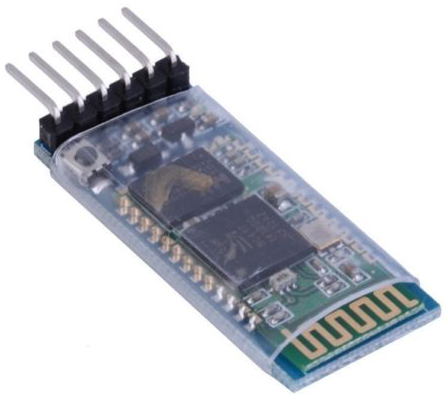
\includegraphics[width=\textwidth]{img/hardware/bluetooth_zs-040.png}
		\caption{Flower one.}
	\end{minipage}
	\hfill
	\begin{minipage}[b]{0.4\textwidth}
		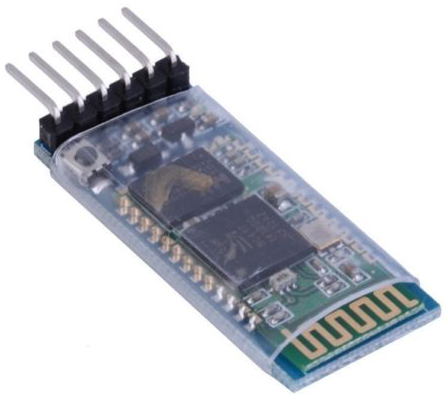
\includegraphics[width=\textwidth]{img/hardware/bluetooth_zs-040.png}
		\caption{Flower two.}
	\end{minipage}
\end{figure}


http://www.instructables.com/id/Modifying-the-AT-Codes-on-a-HC-05-With-the-Code-ZS/


http://www.arduinoecia.com.br/2013/03/modulo-bluetooth-jy-mcu-configuracao.html


Testar ligação com modulo foi usada app bluetooth Terminal HC-05








